\newcommand{\pending}[1]{\textcolor{red}{[#1]}}

\section{Introduction}
\label{sec:intro}

The Air Production Unit (APU) of a Metro do Porto train supplies compressed air to pneumatic consumers such as the secondary suspension. Because the unit has no redundancy, a failure removes the train from service, and the operator requires failures to be detected at least two hours before the train becomes non-operational, with few false alarms \citep{veloso2022metropt}. Our case study addresses this requirement on the public MetroPT-3 dataset \citep{davari2021metropt3data}, which contains 1{,}516{,}948 records of 15 APU signals from February to August 2020 and four air-leak failures documented by maintenance reports.

The previous milestones defined the project and reviewed the literature. The bibliography report concluded that the task is best framed as unsupervised early failure warning, that simple detectors are often competitive with deep models \citep{schmidl2022anomaly}, that point-adjusted metrics can overstate performance \citep{kim2022rigorous}, and that the closest prior study already applies an LSTM autoencoder with SHAP to MetroPT-3 \citep{davari2024explaining}. Our contribution is therefore not a new model but a transparent benchmark: a threshold rule, an Isolation Forest and an LSTM autoencoder compared under one leakage-free protocol with event-level metrics, on data whose quality issues are handled explicitly. A first exploratory analysis found recording gaps covering 17.7\,\% of the period, nine frozen logging segments and a distribution shift between February and the later months.

\subsection{Objectives}
This report covers the first methodology phase. Its objectives are to
\begin{enumerate}[itemsep=2pt]
  \item set out the theoretical framework that supports the proposed solution (Section~\ref{sec:theory});
  \item define the research approach, workflow, data, algorithms and evaluation protocol, and justify the choice of each algorithm (Section~\ref{sec:methods});
  \item present the initial system architecture and the interaction of its components (Section~\ref{sec:architecture});
  \item report a first prototype of the preprocessing pipeline and the Isolation Forest (Section~\ref{sec:prototype}); and
  \item state the main assumptions, limitations and implementation challenges (Section~\ref{sec:assumptions}).
\end{enumerate}
The detailed development of the LSTM autoencoder, the explanation module and the full experiments belong to the second methodology phase.

\section{Theoretical Framework}
\label{sec:theory}

\subsection{Predictive Maintenance as Early Failure Warning}
Predictive maintenance (PdM) monitors the condition of an asset so that interventions are planned when degradation is observed, instead of after a breakdown (corrective maintenance) or at fixed intervals (preventive maintenance) \citep{davari2021survey}. Within PdM, \emph{failure prediction} asks whether a failure will occur within a horizon, while \emph{remaining useful life} estimation predicts the time to the end of life \citep{davari2021survey}. With only four failures, a degradation trajectory cannot be learned, so we formulate the task as \emph{early failure warning}: an alarm should be raised within a fixed horizon before a failure, and not otherwise.

Labelling continuous sensor streams is costly, which makes supervised learning infeasible in railway PdM and motivates treating it as anomaly detection on time series \citep{davari2021survey}. An anomaly is ``an observation that deviates considerably from some concept of normality'' \citep{ruff2021unifying}. In our setting, the concept of normality is learned from a period in which the APU is assumed to work correctly, and every later observation is scored by how far it deviates from that concept. This is a semi-supervised setting in the terminology of \citet{ruff2021unifying}: the training data are assumed to be normal, but no failure labels are used for training.

\subsection{Physical Basis: Compressor Operation and Air Leaks}
\label{sec:physics}
According to the dataset description, the MPG signal starts the compressor \emph{under load} when the pressure falls below 8.2\,bar, so that it delivers air to the reservoirs; otherwise the compressor runs \emph{offloaded} or is switched off, and the description gives motor currents of about 0, 4 and 7\,A for these states. The low-pressure switch (LPS) is activated when the pressure falls below 7\,bar \citep{davari2021metropt3data}. In the data, the motor current shows three clusters at about 0\,A (off), 3.8\,A (offloaded) and 5.4--6.3\,A (under load); we therefore classify a record as \emph{under load} when the motor current exceeds 4.7\,A.

An air leak continuously removes air from the system. To keep the pressure, the compressor must run under load more often and for longer. The share of time under load (the \emph{duty cycle}) is therefore the most direct physical indicator of a leak. Figure~\ref{fig:duty} confirms this in MetroPT-3: averaged over the four failures, the duty cycle is 0.975 during a failure, compared with 0.145 in normal operation. In the 24 hours before a failure, however, it is only 0.161, close to normal. The signature of a leak is strong once the leak is severe and weak beforehand, which is exactly what makes early warning difficult and motivates multivariate detectors that can combine several weak indications (pressures, current, temperature, valve activity).

\begin{figure}[H]
\centering
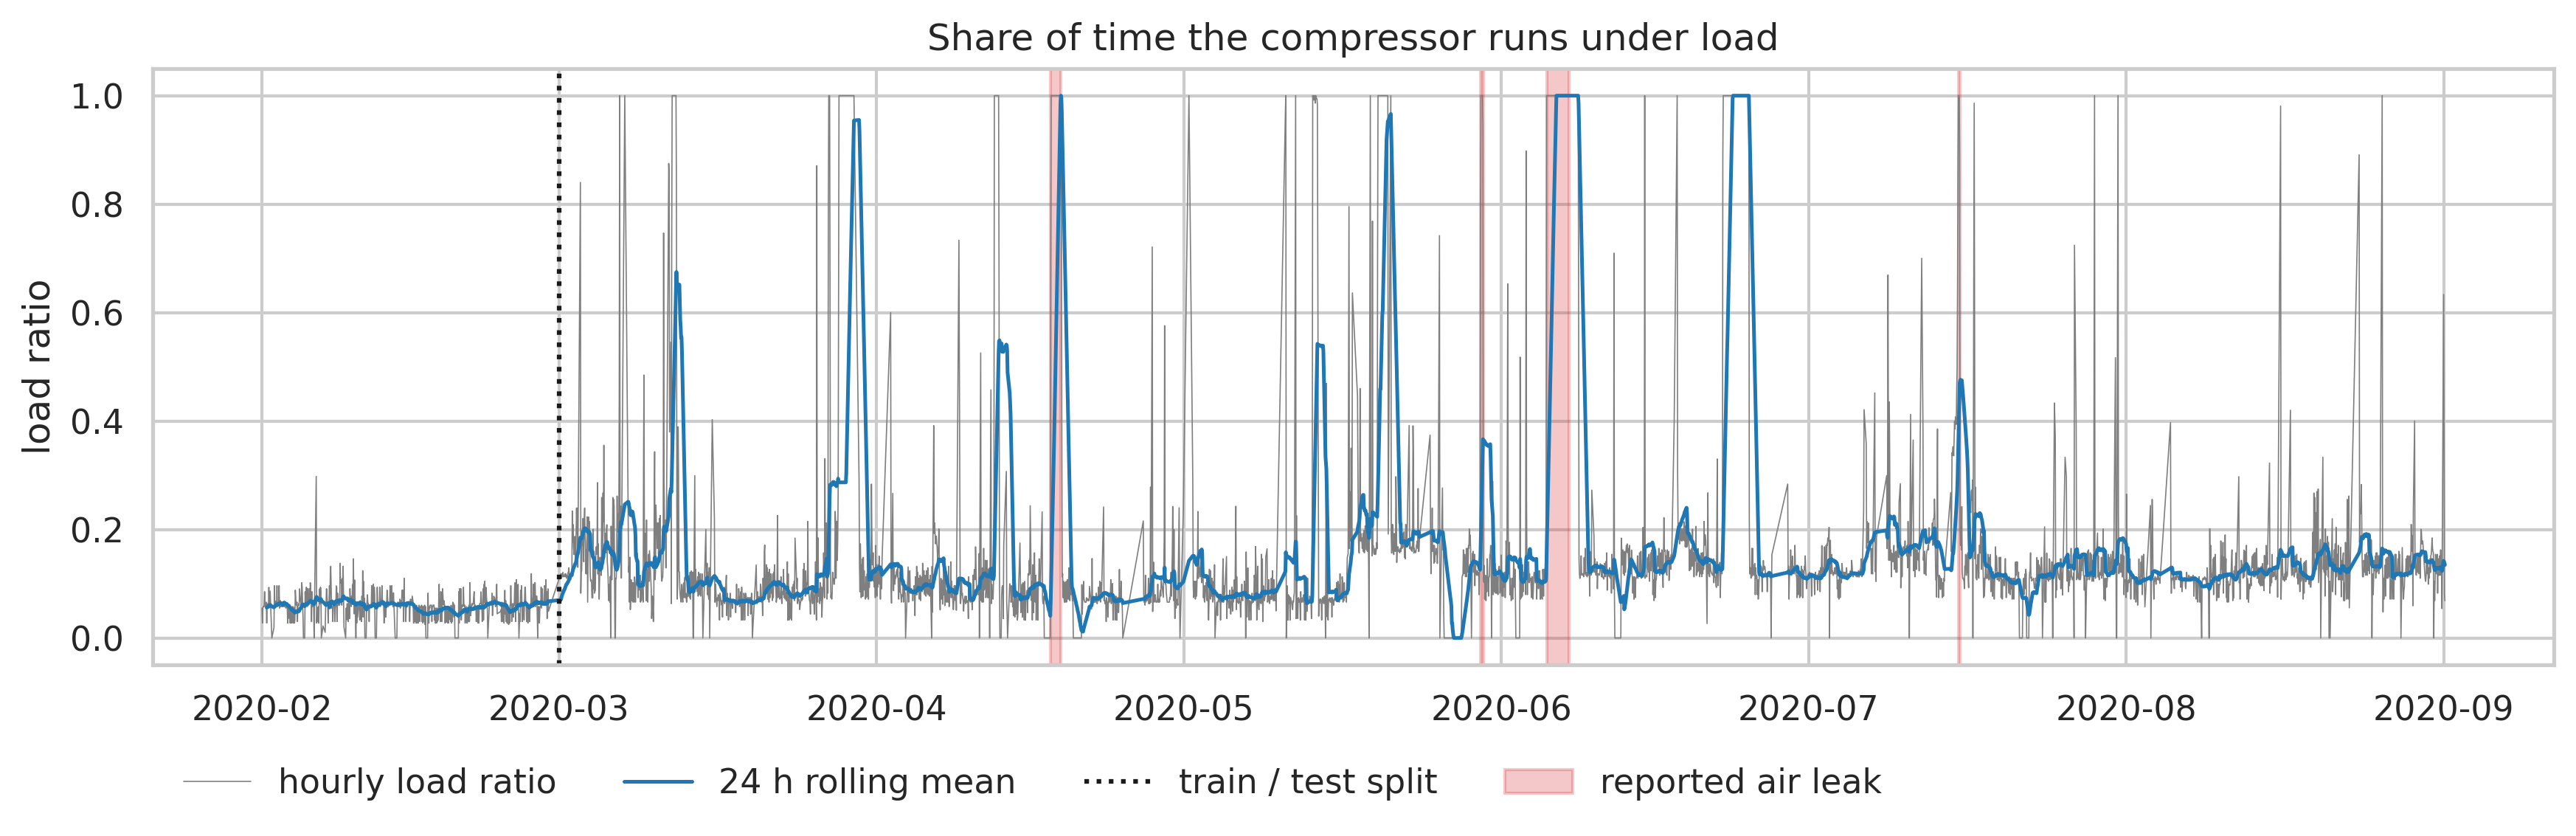
\includegraphics[width=0.9\textwidth]{figures/eda_08_duty_cycle.png}
\caption{Daily share of time under load (motor current $>4.7$\,A). Shaded: reported failures. Source: notebook \texttt{01\_EDA}.}
\label{fig:duty}
\end{figure}

\subsection{Isolation-Based Anomaly Detection}
Isolation Forest \citep{liu2008isolation} does not model normal behaviour explicitly; it isolates individual points. Each tree is built on a random sub-sample by repeatedly choosing a random feature and a random split value between its minimum and maximum, until every point is isolated. Anomalies are few and different, so they are separated after fewer splits and have a shorter path length $h(x)$ from the root. The anomaly score of a point $x$ for a sub-sample size $\psi$ is
\begin{equation}
s(x,\psi) = 2^{-\frac{\mathrm{E}[h(x)]}{c(\psi)}}, \qquad c(\psi) = 2H(\psi-1) - \frac{2(\psi-1)}{\psi},
\label{eq:iforest}
\end{equation}
where $\mathrm{E}[h(x)]$ is the mean path length over all trees, $c(\psi)$ is the average path length of an unsuccessful search in a binary search tree and normalises the score, and $H(i)\approx \ln(i) + 0.5772$ is the harmonic number. Scores close to 1 indicate anomalies; scores well below 0.5 indicate normal points. The method has linear time complexity and low memory requirements and works when the training data contain no anomalies \citep{liu2008isolation}.

\subsection{Reconstruction-Based Detection with LSTM Autoencoders}
An autoencoder learns to compress its input into a low-dimensional representation and to reconstruct the input from it. Trained on normal data only, it reconstructs normal patterns well and unusual patterns poorly, so the reconstruction error serves as an anomaly score; autoencoders can capture nonlinear structure that linear methods such as PCA miss \citep{sakurada2014autoencoders}. For sequences, the encoder and decoder are built from long short-term memory (LSTM) units \citep{hochreiter1997lstm}, which keep information over many time steps. \citet{malhotra2016lstm} train such an LSTM encoder--decoder on normal multi-sensor sequences and use the reconstruction error as the anomaly score. For a sequence $X=(x_1,\dots,x_L)$ with $x_t\in\mathbb{R}^d$ and reconstruction $\hat{X}$, we use the mean squared error
\begin{equation}
e(X) = \frac{1}{L\,d}\sum_{t=1}^{L}\lVert x_t - \hat{x}_t\rVert_2^2 .
\label{eq:recon}
\end{equation}
LSTM autoencoders with a threshold on the reconstruction error are the most common detector in the Metro do Porto literature \citep{silva2023adversarial,gama2024neurosymbolic,davari2024explaining}.

\subsection{From Scores to Alarms}
A continuous score must be turned into a binary decision. Following \citet{silva2023adversarial}, the threshold is the upper outlier fence of the training scores,
\begin{equation}
\tau = Q_3 + k\cdot(Q_3 - Q_1), \qquad k=3,
\label{eq:iqr}
\end{equation}
where $Q_1$ and $Q_3$ are the first and third quartiles. Isolated exceedances are often noise. \citet{ribeiro2016sequential} raise an alarm only for sequences of abnormal observations by passing the binary exceedance signal $x_i\in\{0,1\}$ through a low-pass filter,
\begin{equation}
y_i = y_{i-1} + \alpha\,(x_i - y_{i-1}),
\label{eq:lowpass}
\end{equation}
and signalling an alarm when $y_i > 0.5$, which strongly reduced false alarms in their railway study. Smoothing errors before thresholding to reduce false positives is also used by \citet{hundman2018detecting}, whose operators noted that ``investigation of even a couple false positives can deter users''.

\subsection{Event-Level Evaluation}
Anomaly-detection benchmarks commonly report point-wise precision, recall and F1. For an early-warning system these measures are misleading for two reasons. First, the quantity of interest is whether, and how early, each \emph{failure} is announced, not how many time steps are labelled correctly \citep{lavin2015nab,tatbul2018precision}. Second, the widely used point adjustment, which counts a whole anomalous segment as detected if a single point in it is flagged, lets even random scores reach an F1 of 0.969 on a benchmark where the unadjusted F1 is 0.216 \citep{kim2022rigorous}. Benchmark datasets themselves can also be flawed \citep{wu2021flawed}. We therefore evaluate per failure event and per alarm episode, without point adjustment (Section~\ref{sec:evaluation}).

\subsection{Explainability with Shapley Values}
An alarm is useful only if maintenance staff understand why it was raised; lack of interpretability is a recognised source of mistrust in data-driven PdM \citep{vollert2021interpretable}. SHAP \citep{lundberg2017shap} explains a single prediction $f(x)$ as an additive attribution
\begin{equation}
f(x) = \phi_0 + \sum_{j=1}^{M}\phi_j ,
\label{eq:shap}
\end{equation}
where $\phi_0$ is the expected output over a background data set and $\phi_j$ is the contribution of feature $j$. The $\phi_j$ are Shapley values from cooperative game theory, the unique attribution that satisfies local accuracy, missingness and consistency \citep{lundberg2017shap}. Kernel SHAP estimates them for any model by evaluating it on perturbed inputs. SHAP is the most frequently used explanation method in PdM \citep{cummins2024xpdm}. In our case, $f$ is the anomaly score of a window and the background set is the training period, so $\phi_j$ states how much feature $j$ pushes a window away from typical February behaviour.

\section{Materials and Methods}
\label{sec:methods}

\subsection{Research Approach}
The study is a quantitative, experimental comparison. Three detectors of increasing complexity are applied to the same data under the same protocol:
\begin{enumerate}[itemsep=2pt]
  \item a \textbf{threshold rule} that encodes the physical leak signature directly (milestone 2);
  \item an \textbf{Isolation Forest}, a fast, shallow multivariate detector; and
  \item an \textbf{LSTM autoencoder}, a deep sequence model.
\end{enumerate}
All three share the preprocessing and the evaluation; the two learned detectors also share the alarm logic. The detector is therefore the only independent variable, and differences in the results can be attributed to it. A second, smaller comparison (ablation) repeats the learned detectors without removing frozen segments, to measure the effect of the data-quality handling.

\subsection{Workflow}
Figure~\ref{fig:workflow} shows the workflow. Steps~1--4 are common to all detectors, steps~5--6 are detector-specific, and steps~7--8 are again common.

\begin{figure}[H]
\centering
\begin{tikzpicture}[
  box/.style={draw, rounded corners=2pt, align=center, minimum width=2.8cm, minimum height=1.05cm, font=\small},
  common/.style={box, fill=blue!6},
  model/.style={box, fill=orange!12},
  arr/.style={-{Stealth[length=2.2mm]}, thick}]
\node[common] (a) {1. Download\\ \& load data};
\node[common, right=0.4cm of a] (b) {2. Remove frozen\\ segments};
\node[common, right=0.4cm of b] (c) {3. Gap-aware\\ 10-min windows};
\node[common, right=0.4cm of c] (d) {4. Chronological split\\ \& train-only scaling};
\node[model, below=0.9cm of d] (e) {5. Fit detector\\ on February};
\node[model, left=0.4cm of e] (f) {6. Anomaly score\\ per window};
\node[common, left=0.4cm of f] (g) {7. Threshold\\ + low-pass filter};
\node[common, left=0.4cm of g] (h) {8. Event-level\\ evaluation};
\node[box, fill=green!8, below=0.9cm of g] (i) {9. SHAP explanation\\ of each alarm};
\draw[arr] (a)--(b); \draw[arr] (b)--(c); \draw[arr] (c)--(d); \draw[arr] (d)--(e);
\draw[arr] (e)--(f); \draw[arr] (f)--(g); \draw[arr] (g)--(h); \draw[arr] (g)--(i);
\end{tikzpicture}
\caption{Workflow. Blue: shared by all detectors; orange: detector-specific; green: explanation (phase~2).}
\label{fig:workflow}
\end{figure}

\subsection{Data and Inputs}
\label{sec:data}
\paragraph{Source.} MetroPT-3 \citep{davari2021metropt3data} is downloaded by a script from the UCI Machine Learning Repository (CC BY 4.0) and is never stored in the repository. The four failure periods published on the dataset page are the only ground truth. Table~\ref{tab:signals} lists the signals and how each one is used.

\begin{table}[H]
\centering
\small
\caption{MetroPT-3 signals (descriptions from the dataset page) and their use in this study.}
\label{tab:signals}
\begin{tabular}{llll}
\toprule
Signal & Description & Unit / type & Use \\
\midrule
TP2 & Pressure on the compressor & bar & feature \\
TP3 & Pressure at the pneumatic panel & bar & feature \\
H1 & Pressure drop at cyclonic separator filter & bar & feature \\
DV\_pressure & Pressure drop at air-dryer tower discharge & bar & feature \\
Reservoirs & Downstream reservoir pressure & bar & feature \\
Oil\_temperature & Compressor oil temperature & $^\circ$C & feature \\
Motor\_current & Current of one motor phase & A & feature, load state \\
COMP & Air intake valve & binary & feature \\
DV\_electric & Compressor outlet valve & binary & feature \\
Towers & Active air-drying tower & binary & feature \\
MPG & Starts compressor under load ($<8.2$ bar) & binary & feature \\
LPS & Low-pressure switch ($<7$ bar) & binary & evaluation reference \\
Pressure\_switch & Discharge in the air-drying towers & binary & feature \\
Oil\_level & Oil below expected level & binary & feature \\
Caudal\_impulses & Air-flow pulse counter & binary & feature \\
\bottomrule
\end{tabular}
\end{table}

LPS is deliberately excluded from the inputs. It is a symptom of low pressure that already reflects a developing failure, and the operator-oriented criterion of \citet{silva2023adversarial} measures early warning relative to it; using it as a feature would make the evaluation circular.

\paragraph{Input variables.} For each 10-minute window, the model input consists of the mean, standard deviation, minimum and maximum of the seven analogue signals (28 features), the share of active time of the seven digital signals other than LPS (7 features) and the share of time under load (1 feature), i.e.\ 36 features. The LSTM autoencoder will additionally use the scaled raw signals within each window as a sequence (Section~\ref{sec:lstm}).

\paragraph{Output variables.} For every window the system produces (i) an anomaly score, (ii) a binary alarm and, for alarms, (iii) a ranked list of the features that contribute most to the score. For every failure, the evaluation produces a detection flag and the lead time.

\paragraph{Split.} February 2020 (windows ending on or before 1~March 2020) is the training period; March to August 2020 is the test period, which contains all four failures. Taking the first month as normal training data and the following months as test data follows \citet{silva2023adversarial}. No information from the test period is used for training, scaling or setting thresholds.

\subsection{Preprocessing}
\label{sec:preprocessing}
\begin{enumerate}[itemsep=3pt]
  \item \textbf{Frozen segments.} Segments in which all seven analogue signals keep exactly the same value for at least 30 minutes are removed. Under operation at least one pressure or temperature changes within minutes, so such segments indicate a stuck logger. Nine segments (3.3\,\% of records) were found, one of them in the 15 hours before failure~1 (Figure~\ref{fig:frozen}).
  \item \textbf{Gap-aware windows.} Records are aggregated into windows $[t-10\,\text{min},\,t)$ indexed by the end time $t$, the earliest moment at which a decision can be made, so lead times are not inflated by the window length. A window is kept only if it contains at least 50\,\% of the expected 60 records; gaps are not filled with interpolated values.
  \item \textbf{Chronological split} as described above.
  \item \textbf{Scaling.} Each feature is standardised with the mean and standard deviation of the training windows only.
\end{enumerate}

\begin{figure}[H]
\centering
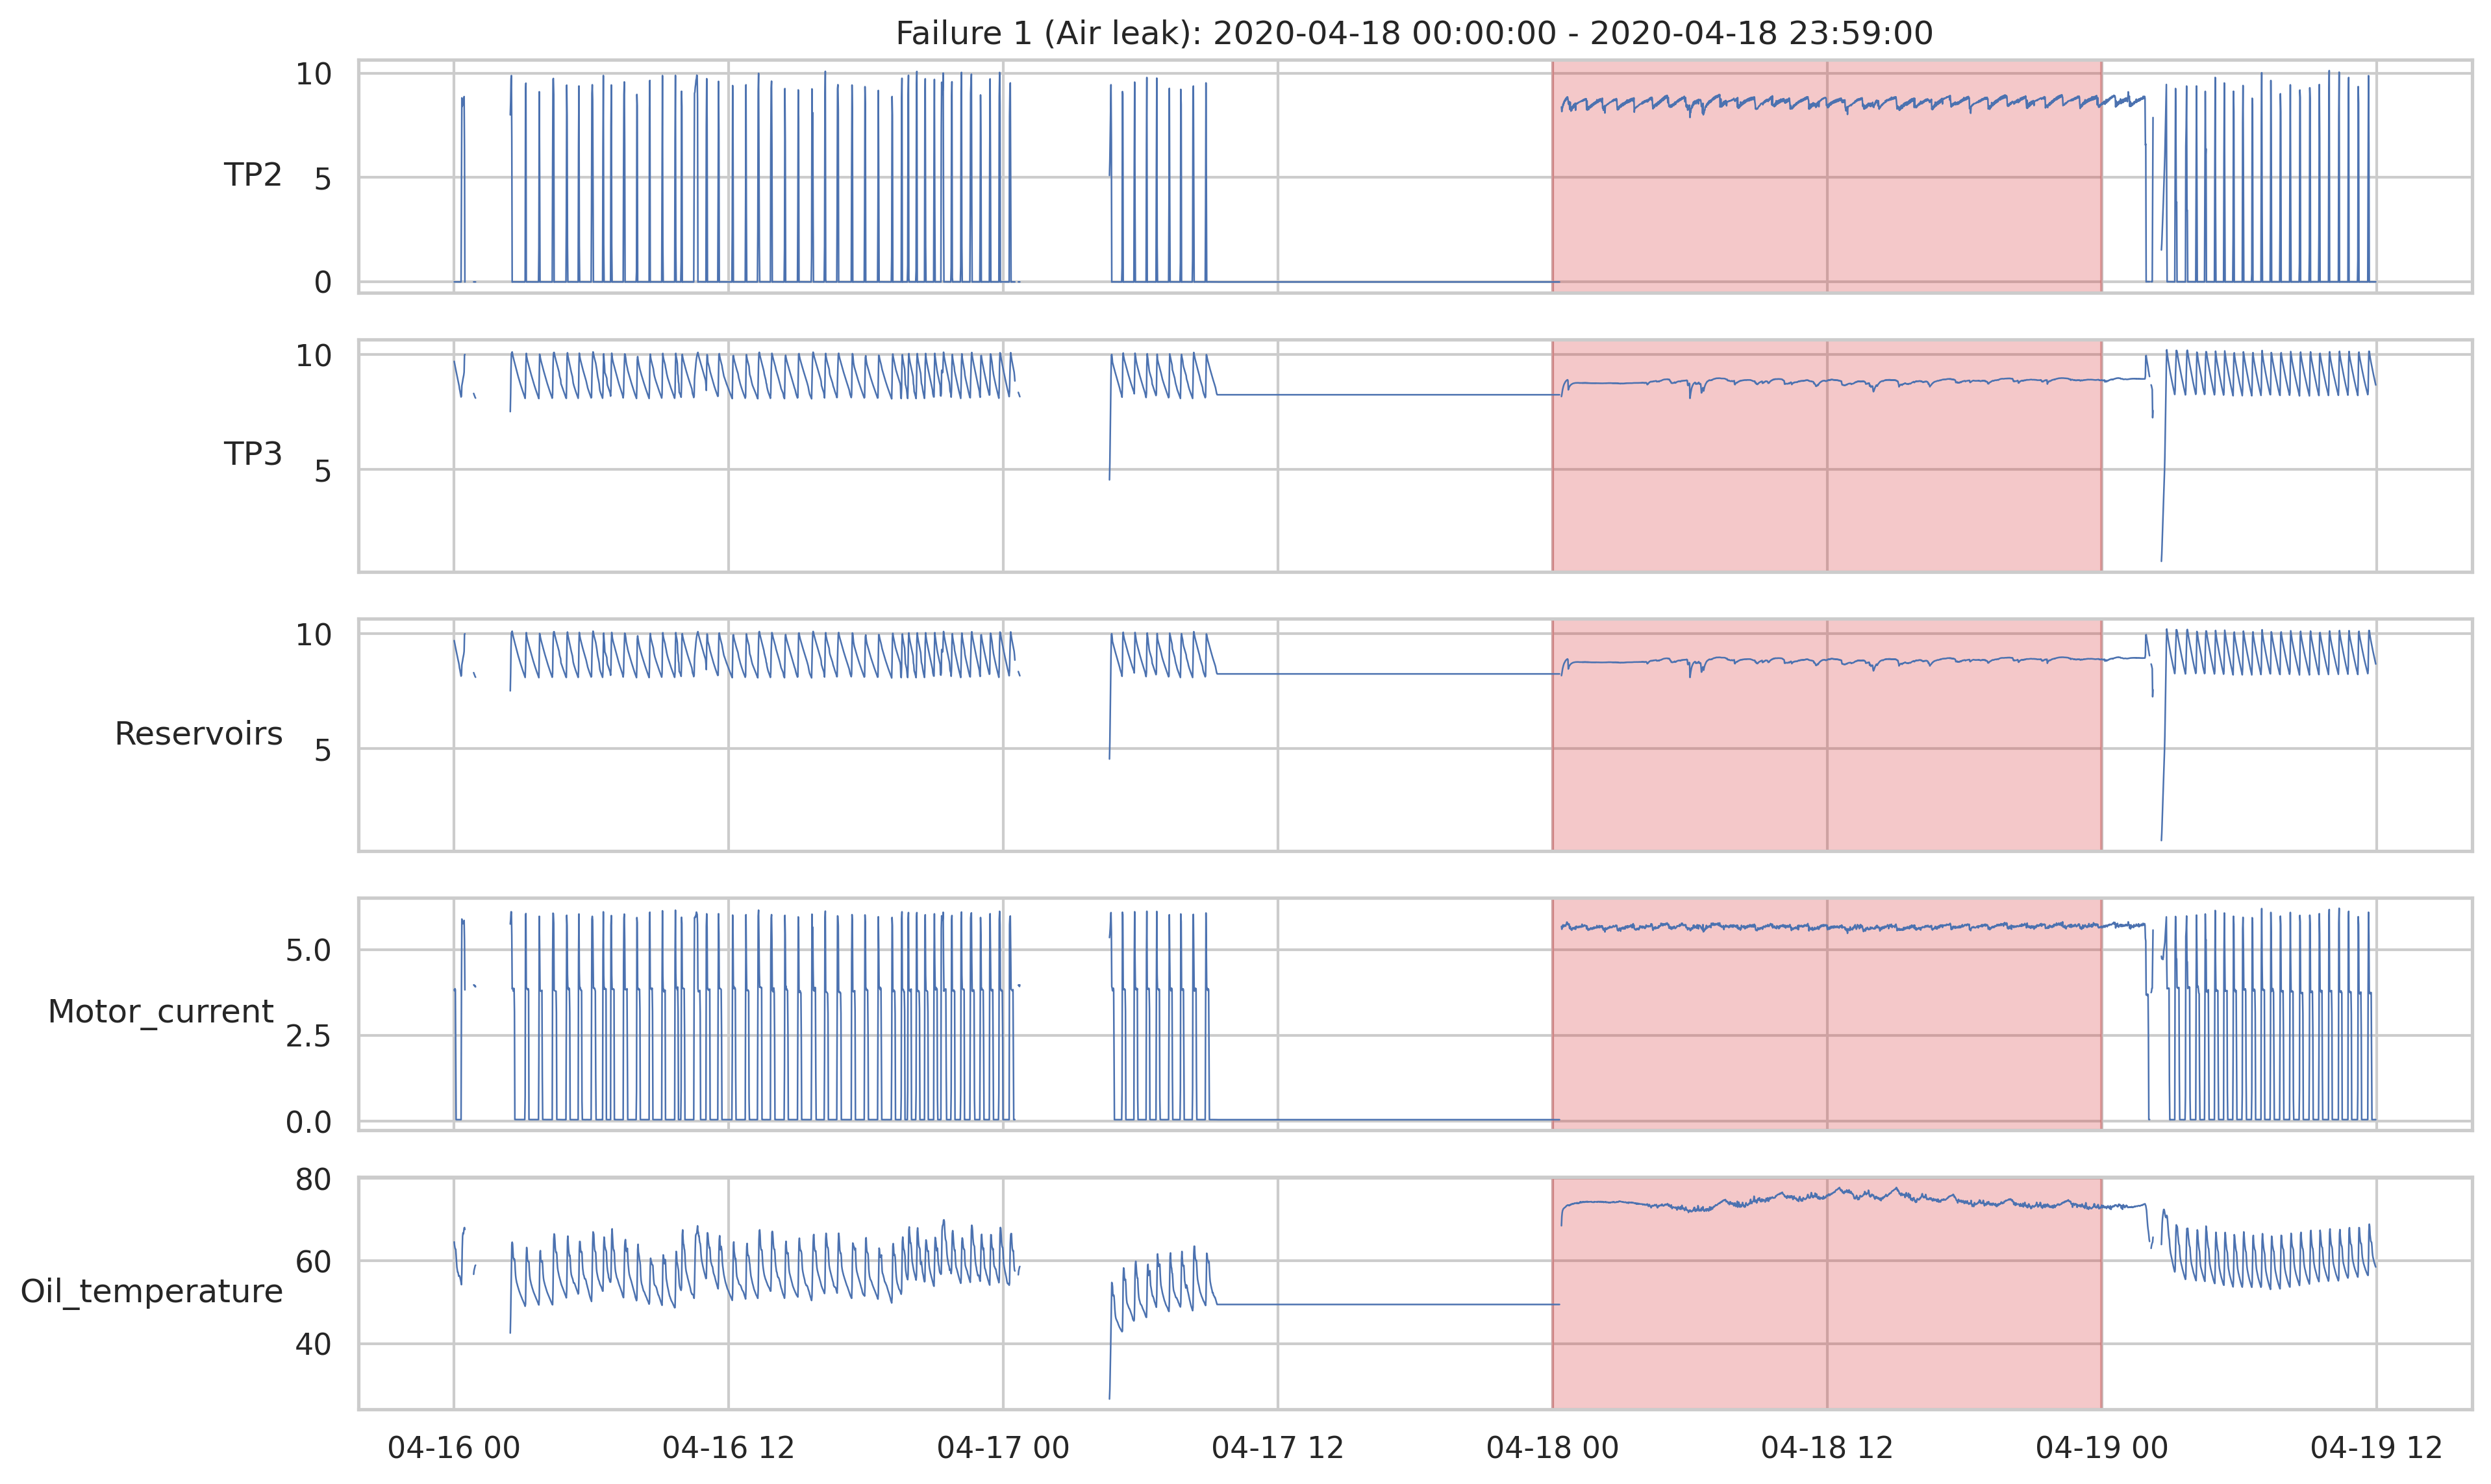
\includegraphics[width=0.85\textwidth]{figures/eda_07_failure_1_zoom.png}
\caption{Signals around failure 1. All signals are flat from 17~April 09:20 to 18~April 00:18 (frozen logging). Source: notebook \texttt{01\_EDA}.}
\label{fig:frozen}
\end{figure}

\subsection{Algorithms and Reasons for Their Selection}
Table~\ref{tab:algorithms} summarises the selected algorithms and why each was chosen.

\begin{table}[H]
\centering
\small
\caption{Selected algorithms and reasons for selection.}
\label{tab:algorithms}
\begin{tabular}{p{2.6cm}p{4.3cm}p{7.3cm}}
\toprule
Algorithm & Principle & Reasons for selection \\
\midrule
Threshold rule & Training quantiles of four physically motivated window features; at least 2 of 4 rules for 3 consecutive windows & Directly encodes the leak signature (Section~\ref{sec:physics}); fully interpretable; lower bound that learned models must beat. \\
\addlinespace
Isolation Forest \citep{liu2008isolation} & Anomalies are isolated by fewer random splits (Eq.~\ref{eq:iforest}) & Multivariate, trained on normal data only, fast and with few hyper-parameters; simple methods are often competitive with deep models \citep{schmidl2022anomaly}; represents the ``simple'' side of gap~G2. \\
\addlinespace
LSTM autoencoder \citep{malhotra2016lstm} & Reconstruction error of normal sequences (Eq.~\ref{eq:recon}) & Models temporal dependencies within a window; standard detector in the APU literature \citep{silva2023adversarial,gama2024neurosymbolic}, including on MetroPT-3 \citep{davari2024explaining}; makes our results comparable. \\
\addlinespace
Threshold $Q_3+3\,\mathrm{IQR}$ + low-pass filter & Eq.~\ref{eq:iqr} and \ref{eq:lowpass} & Uses training scores only; suppresses isolated exceedances; same rule for both learned detectors, as used in \citep{silva2023adversarial,ribeiro2016sequential}. \\
\addlinespace
Kernel SHAP \citep{lundberg2017shap} & Shapley-value attribution of the anomaly score (Eq.~\ref{eq:shap}) & Model-agnostic, so the same explanation method applies to both learned detectors; most used method in explainable PdM \citep{cummins2024xpdm}. \\
\bottomrule
\end{tabular}
\end{table}

Alternatives were considered and not selected. Supervised classifiers would need labelled failures for training, and only four exist. Distance- and density-based detectors such as nearest-neighbour methods were not selected because Isolation Forest offers linear time complexity and low memory use, and compared favourably with such methods in its original evaluation \citep{liu2008isolation}. Generative adversarial models performed best in \citet{silva2023adversarial}, but are harder to train and tune; for a benchmark whose aim is a fair comparison of a simple and a deep model, the LSTM autoencoder is the established representative.

\subsection{Initial Design of the LSTM Autoencoder}
\label{sec:lstm}
The LSTM autoencoder receives, for each 10-minute window, the sequence of the scaled raw analogue and digital signals (without LPS) at their native resolution of about 10\,s, i.e.\ a sequence of up to 60 steps with 14 channels. Windows with less than 50\,\% coverage are skipped, as for the window features. The initial architecture is symmetric: an encoder with two LSTM layers (64 and 16 units) compresses the sequence into a 16-dimensional representation, which is repeated over the sequence length and decoded by two LSTM layers (16 and 64 units) and a linear output layer to the 14 channels. The model is trained with the mean squared error (Eq.~\ref{eq:recon}) and the Adam optimiser; the last 20\,\% of February are held out chronologically for early stopping. The anomaly score of a window is its reconstruction error, which then passes through the same alarm logic as the Isolation Forest score. Layer sizes, sequence representation and training settings will be finalised in the second phase.

\subsection{Alarm Logic}
For the learned detectors, the threshold $\tau$ is computed from the training scores with Eq.~\ref{eq:iqr} ($k=3$). The exceedance signal $x_i=\mathbf{1}[s_i>\tau]$ is filtered with Eq.~\ref{eq:lowpass} using $\alpha=0.3$; with this value, two consecutive exceeding windows are needed for a first alarm. The filter is reset to zero after a recording gap, so windows on either side of a gap are never treated as consecutive. The threshold rule keeps its own persistence filter (three consecutive windows) from milestone 2.

\subsection{Evaluation Protocol}
\label{sec:evaluation}
The evaluation is applied identically to all detectors on the test period with a warning horizon of $h=2$\,h, the operator requirement \citep{veloso2022metropt}.
\begin{itemize}[itemsep=2pt]
  \item \textbf{Detection.} A failure with reported start $t_s$ and end $t_e$ is detected if an alarm occurs in $[t_s-h,\,t_e]$.
  \item \textbf{Lead time.} $t_s - t_a$ in minutes, where $t_a$ is the first alarm in that interval; positive values are early warnings, negative values are detection delays.
  \item \textbf{Lead time relative to LPS.} The same difference measured to the first LPS activation in $[t_s-h,\,t_e]$, corresponding to the criterion of \citet{silva2023adversarial}.
  \item \textbf{False alarms.} Consecutive alarm windows form an episode; episodes that do not overlap any interval $[t_s-h,\,t_e]$ are false alarms, reported as a count and per day.
  \item \textbf{Window-level precision, recall and F1} without point adjustment, as a secondary view.
\end{itemize}
Because there are only four failures, results are reported per failure rather than only as averages.

\subsection{Reproducibility}
All code is written in Python with pinned package versions (\texttt{requirements.txt}) and a fixed random seed (42). The dataset is downloaded by \texttt{scripts/download\_data.py}. All notebooks can be run on Google Colab, where the first cell clones the repository and downloads the data. Code and results are available at \url{https://github.com/mohamedfarez/IntelligentSystemsCaseStudy}.

\section{System Architecture}
\label{sec:architecture}
The system is organised in five layers (Figure~\ref{fig:architecture}). Each layer is a Python module with a small interface, so detectors can be exchanged without changing the rest of the pipeline. Table~\ref{tab:modules} maps the components to the code.

\begin{figure}[H]
\centering
\begin{tikzpicture}[
  layer/.style={draw, rounded corners=3pt, text width=15.0cm, minimum height=0.95cm, align=center, font=\small, inner sep=5pt},
  arr/.style={-{Stealth[length=2mm]}, thick}]
\node[layer, fill=gray!8] (L1) {\textbf{Data layer:} UCI download $\cdot$ loading $\cdot$ quality checks};
\node[layer, fill=blue!6, below=0.4cm of L1] (L2) {\textbf{Preprocessing:} frozen-segment mask $\cdot$ gap-aware windows $\cdot$ chronological split $\cdot$ train-only scaler};
\node[layer, fill=orange!12, below=0.4cm of L2] (L3) {\textbf{Detectors:} threshold rule $\cdot$ Isolation Forest $\cdot$ LSTM autoencoder};
\node[layer, fill=blue!6, below=0.4cm of L3] (L4) {\textbf{Alarm logic:} $Q_3+3\,\mathrm{IQR}$ threshold $\cdot$ low-pass filter};
\node[layer, fill=green!8, below=0.4cm of L4] (L5) {\textbf{Evaluation \& explanation:} event-level KPIs $\cdot$ SHAP};
\draw[arr] (L1.south)--(L2.north); \draw[arr] (L2.south)--(L3.north);
\draw[arr] (L3.south)--(L4.north); \draw[arr] (L4.south)--(L5.north);
\end{tikzpicture}
\caption{System architecture. Each layer only uses the output of the layer above.}
\label{fig:architecture}
\end{figure}

\begin{table}[H]
\centering
\small
\caption{Components, code modules and interfaces.}
\label{tab:modules}
\begin{tabular}{p{2.6cm}p{5.0cm}p{7.3cm}}
\toprule
Component & Module & Interface (input $\rightarrow$ output) \\
\midrule
Configuration & \texttt{src/config.py} & Paths, schema, seed, failure periods, split date \\
Data loading & \texttt{src/data\_loading.py} & CSV $\rightarrow$ time-indexed frame; quality report \\
Preprocessing & \texttt{src/preprocessing.py} & Raw frame $\rightarrow$ scaled train / test windows \\
Threshold rule & \texttt{src/threshold\_baseline.py} & Window features $\rightarrow$ alarms \\
Learned detectors & \texttt{src/detectors.py} & \texttt{fit(train)}; \texttt{score(X)} $\rightarrow$ score per window \\
Alarm logic & \texttt{src/alarm\_logic.py} & \texttt{fit(train scores)}; \texttt{predict(scores)} $\rightarrow$ alarms \\
Evaluation & \texttt{src/evaluation.py} & Alarms $\rightarrow$ per-failure table and KPIs \\
Experiment runner & \texttt{src/run\_experiment.py} & Raw frame + detector name $\rightarrow$ all results \\
Explanation (phase 2) & \texttt{src/explain.py} & Detector + alarm windows $\rightarrow$ SHAP values \\
\bottomrule
\end{tabular}
\end{table}

The components interact in one direction only. The preprocessing never sees detector outputs, the alarm logic is fitted on training scores only, and the evaluation receives nothing but the alarm series and the failure periods. This separation makes leakage from the test period structurally impossible and guarantees that all detectors are evaluated by the same code.

\section{Initial Prototype}
\label{sec:prototype}
The preprocessing pipeline, the Isolation Forest, the common alarm logic and the shared evaluation are implemented (notebook \texttt{02\_preprocessing\_iforest}). The Isolation Forest uses 200 trees, a sub-sample size of 256 as recommended by \citet{liu2008isolation} and the fixed seed. No parameter was tuned on the test period.

\paragraph{Verification.} Before the run on the real data, the code was checked in three ways. (i) The evaluation functions were moved from the threshold baseline into a shared module; the baseline was re-run and produced identical results. (ii) The pipeline was run on a synthetic data set with the same schema, sampling interval and period as MetroPT-3, containing four simulated leaks, a recording gap and an inserted frozen segment before the first leak. The frozen segment was found and removed, and all four simulated leaks were detected. (iii) Without frozen-segment removal, the inserted frozen segment before the first simulated leak produced an apparent early warning of 120 minutes that disappeared once the segment was removed. On synthetic data this shows that frozen data can create alarms that look like early warnings but are caused by the logger, not by the machine.

\paragraph{Results on MetroPT-3.} After frozen-segment removal (nine segments, 50{,}716 records, 3.3\,\%), 24{,}235 windows remain: 3{,}552 for training and 20{,}683 for testing. The threshold computed from the February scores is $\tau=0.637$; 9.8\,\% of the test windows exceed it. Table~\ref{tab:proto} compares the Isolation Forest with the threshold rule of milestone~2 under the shared evaluation, and Table~\ref{tab:lead} gives the lead time per failure. The baseline values are identical to those reported in milestone~2.

\begin{table}[H]
\centering
\small
\caption{Prototype results on the test period (March--August 2020), horizon 2\,h. IF = Isolation Forest.}
\label{tab:proto}
\begin{tabular}{lccc}
\toprule
Metric & Threshold rule & IF & IF, no frozen mask \\
\midrule
Failures detected & 4 / 4 & 4 / 4 & 4 / 4 \\
Early warnings (before start) & 1 & 1 & 1 \\
Median lead time [min] & $-20$ & $-5$ & $-5$ \\
False-alarm episodes & 45 & 96 & 100 \\
False alarms per day & 0.245 & 0.522 & 0.543 \\
Window precision & 0.324 & 0.421 & 0.290 \\
Window recall & 0.911 & 0.947 & 0.921 \\
Window F1 & 0.478 & 0.583 & 0.442 \\
\bottomrule
\end{tabular}
\end{table}

\begin{table}[H]
\centering
\small
\caption{Lead time per failure in minutes (positive = before the reported start) and first LPS activation within $[t_s-2\,\text{h},\,t_e]$.}
\label{tab:lead}
\begin{tabular}{cccccc}
\toprule
Failure & Threshold rule & IF & IF, no mask & First LPS activation & IF lead vs.\ LPS \\
\midrule
1 & $-50$ & $-40$ & $-40$ & none & -- \\
2 & $-20$ & $0$ & $0$ & none & -- \\
3 & $-20$ & $-10$ & $-10$ & 06 Jun, 19:42 & 33.5\,h \\
4 & $+120$ & $+120$ & $+120$ & 15 Jul, 17:20 & 4.8\,h \\
\bottomrule
\end{tabular}
\end{table}

\begin{figure}[H]
\centering
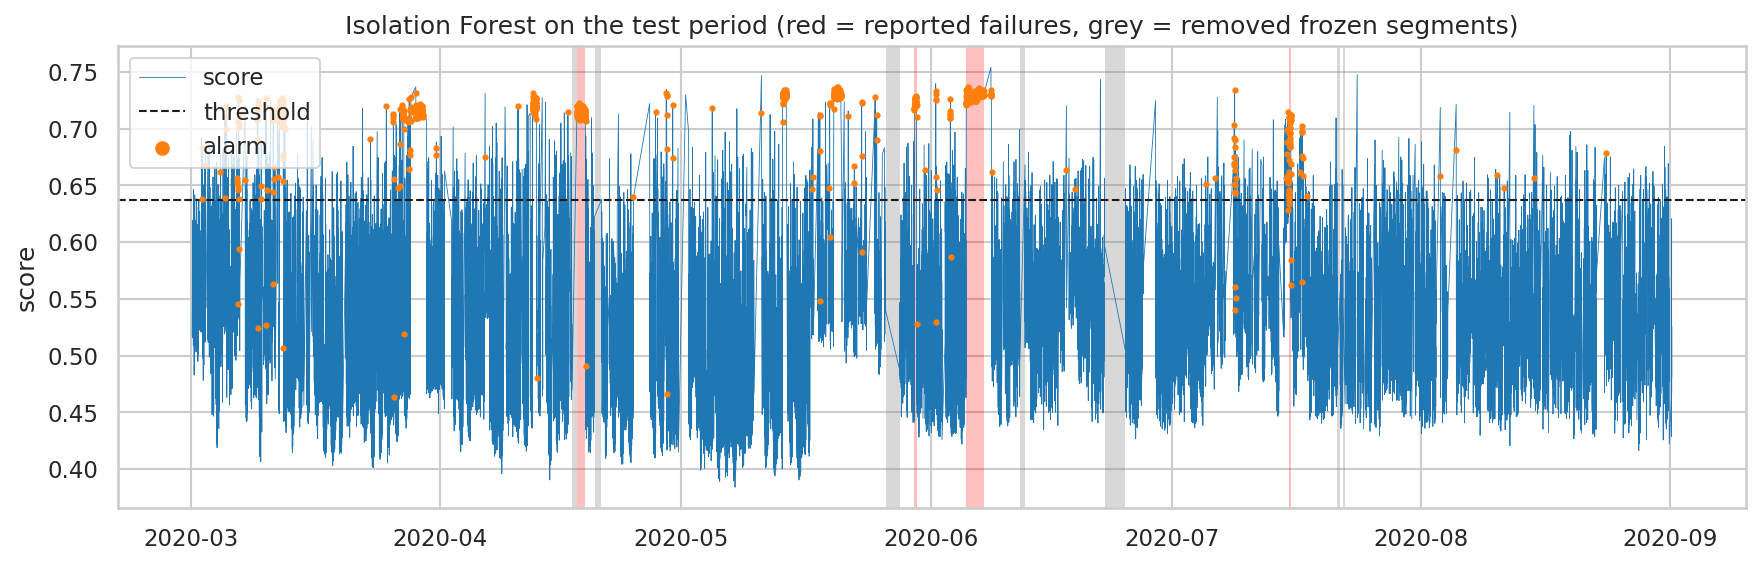
\includegraphics[width=\textwidth]{figures/iforest_02_alarms_test_period.png}
\caption{Isolation Forest scores and alarms on the test period. Red: reported failures; grey: removed frozen segments.}
\label{fig:iforest}
\end{figure}

Four observations follow. First, the Isolation Forest detects every failure and does so 10 to 20 minutes earlier than the threshold rule for failures 1--3; like the threshold rule, it warns two hours ahead only for failure~4. Second, it produces about twice as many false-alarm episodes (0.52 instead of 0.25 per day), many of them short and scattered over the summer (Figure~\ref{fig:iforest}), even though its window-level precision and F1 are higher. Judged only by the window-level F1, the Isolation Forest would appear clearly better; the event-level view shows the cost for maintenance staff. This illustrates why the evaluation protocol reports episodes per day. Third, removing frozen segments does not change any lead time on the real data, but it raises the window precision from 0.290 to 0.421 and removes four false-alarm episodes, mainly from the long frozen segment in late June. Fourth, the low-pressure switch did not activate within the evaluation interval of failures~1 and~2 and activated only about 34 hours after the reported start of failure~3. An evaluation that relies only on the ``two hours before LPS'' criterion would therefore have no reference point for half of the MetroPT-3 failures, which supports reporting both reference points.

The main cause of the false alarms is the distribution shift between February and the later months (Section~\ref{sec:assumptions}). Figure~\ref{fig:shift} shows the mean of each scaled test feature: the minimum compressor pressure (\texttt{TP2\_min}) lies on average 67 training standard deviations away from its February mean. In February the compressor stops in almost every 10-minute window, so the minimum pressure is close to zero with very little variance; in summer, windows in which the compressor runs under load throughout occur more often. The Isolation Forest is not affected by the scaling itself, because its random splits are drawn between the minimum and maximum of each feature, but the shifted test windows lie outside the February range and are isolated quickly. Any change to the features or the training period to address this will be justified by this analysis of the training data and not selected on the test failures.

\begin{figure}[H]
\centering
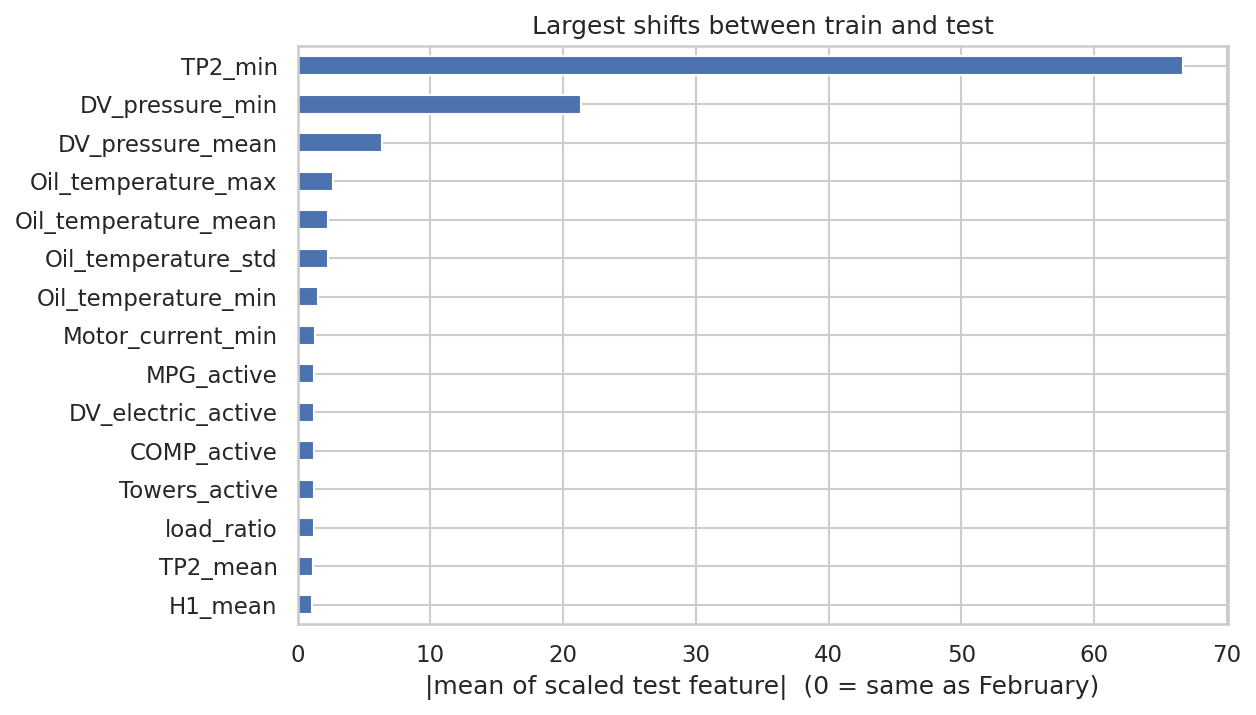
\includegraphics[width=0.72\textwidth]{figures/prep_02_feature_shift.png}
\caption{Absolute mean of the scaled test features (0 = same as February). The 15 largest shifts are shown.}
\label{fig:shift}
\end{figure}

\section{Assumptions and Challenges}
\label{sec:assumptions}

\subsection{Assumptions}
\begin{enumerate}[itemsep=2pt]
  \item \textbf{February is normal.} The training month contains no reported failure and is assumed to represent normal operation. Unreported faults in February would raise the thresholds and reduce sensitivity.
  \item \textbf{The maintenance reports are correct and complete.} Only the four published failure periods count as failures. Their start times are the reported times, not the physical onset of the leaks; the thesis of \citet{barros2020thesis} even dates failure~4 two days later than the dataset page.
  \item \textbf{Frozen segments are logging artefacts}, not real machine states, and can be removed.
  \item \textbf{Ten-minute windows} are short enough to react within the two-hour horizon and long enough to contain several compressor cycles.
\end{enumerate}

\subsection{Limitations and Challenges}
\begin{enumerate}[itemsep=2pt]
  \item \textbf{Four failures.} Every failure changes the event recall by 25 percentage points, so differences between detectors must be interpreted with care and are reported per failure.
  \item \textbf{Weak early signal.} The leak signature is strong during a failure but weak one day before (Section~\ref{sec:physics}); some failures may only be detectable after their reported start.
  \item \textbf{Distribution shift.} February has a lower duty cycle and oil temperature than the later months. The prototype confirms that a detector trained on February flags parts of normal summer operation (Section~\ref{sec:prototype}). For the LSTM autoencoder, features with almost no variance in February, such as \texttt{TP2\_min}, will also dominate the reconstruction error after standardisation; robust scaling or removing such features will be examined. We keep February as the only training month to avoid leakage and report the shift as a limitation; it is a change in the input distribution rather than concept drift in the supervised sense \citep{gama2014drift}.
  \item \textbf{Recording gaps} (17.7\,\% of the period) shorten the usable data and can hide the onset of a failure.
  \item \textbf{Threshold sensitivity.} Window length, the IQR factor and the filter constant influence lead time and false alarms. They are fixed in advance here; their sensitivity will be studied in phase~2 without selecting values on the test failures.
  \item \textbf{Computation.} The LSTM autoencoder requires a GPU for reasonable training times; Google Colab is used.
  \item \textbf{Explanation cost.} Kernel SHAP requires many model evaluations; explanations are therefore computed only for alarm windows, with a sample of February windows as background.
\end{enumerate}

\section{Conclusion}
\label{sec:conclusion}
This report defined the theoretical and methodological basis of our case study. Early warning of air leaks is formulated as unsupervised anomaly detection on windows of APU sensor data, motivated by the physical leak signature of a compressor that runs under load almost continuously during a failure. Three detectors of increasing complexity, a threshold rule, an Isolation Forest and an LSTM autoencoder, share one preprocessing pipeline that removes frozen logging segments and respects recording gaps, one alarm logic, and one event-level evaluation with lead time, false alarms per day and lead time relative to the low-pressure signal. The modular architecture separates data, preprocessing, detection, alarm logic and evaluation, which prevents leakage and guarantees that all detectors are judged by the same code. A first prototype shows that the Isolation Forest detects all four failures and reacts earlier than the threshold rule for three of them, but raises about twice as many false alarms, mainly because of the distribution shift between February and the summer months; it also shows that the low-pressure switch is not a usable reference for two of the four failures.

The second methodology phase will implement the LSTM autoencoder and the SHAP explanation module, define the experimental scenarios (detector comparison, frozen-segment ablation and parameter sensitivity) and run the full evaluation.
